\documentclass{article}

% set font encoding for PDFLaTeX or XeLaTeX
\usepackage{ifxetex}
\ifxetex
  \usepackage{fontspec}
\else
  \usepackage[T1]{fontenc}
  \usepackage[utf8]{inputenc}
  \usepackage{lmodern}
  \usepackage{graphicx}
  \usepackage{float}

\fi

% used in maketitle
\title{Tiro Parabólico\\(Trayectoria)}
\author{David Hndz\\ Universidad de Sonora\\ Lic. en Física}

% Enable SageTeX to run SageMath code right inside this LaTeX file.
% documentation: http://mirrors.ctan.org/macros/latex/contrib/sagetex/sagetexpackage.pdf
% \usepackage{sagetex}

\begin{document}
\maketitle
\section {¿Qué hice?}
El código que programamos se basó principalmente en el aprendizaje del comando de repetición (sumatoria) DO y el comando de condición IF , los cuales tienen características particulares aún no vistas pero como se mencionó anteriormente se nos enseñó lo básico de estos.
También se nos enseñó a utilizar el graficador Gnupot
\section{introducción}
\subsection{DO}
Este comando tiene la función de Sumatoria. El ciclo DO es usado para repetir un conjunto de sentencias una determinada cantidad de veces.
\begin{verbatim}
Se muestra el siguiente ejemplo donde se calcula la suma de los enteros desde el 1
hasta n (suponiendo que a n se le ha asignado un valor previamente):
      integer i, n, suma
      :
      :
      :
      suma = 0
      do 10 i = 1, n
         suma = suma + i
         write(*,*) 'i =', i
         write(*,*) 'suma =', suma
   10 continue

El número 10 es una sentencia de etiqueta. Típicamente, podría haber varios ciclos y
otras sentencias en un programa que requieran una sentencia de etiqueta.

El programador es responsable de asignar un número único a cada etiqueta 
en cada programa (o subprograma). 
Recordar que las posiciones de las columnas 2-5 son reservadas 
para sentencias de etiquetas. El valor numérico de las sentencias de etiqueta 
no tienen ningún significado, por lo que cualquier valor entero puede ser usado. 
Por lo general, los programadores incrementan las etiquetas de 10 en 10 cada vez.
La variable en la sentencia do es incrementada en 1 por default. 
Sin embargo, se puede usar cualquier otro entero para el paso o incremento. 
El siguiente segmento de programa muestra los números pares en forma decreciente 
entre el 1 y 10:

      integer i

      do 20 i = 10, 1, -2
         write(*,*) 'i =', i
   20 continue
La forma general del ciclo do es la siguiente:

      do etiqueta  var =  expr1, expr2, expr3
         sentencias
 etiq continue
donde:
var es la variable del ciclo (conocida con frecuencia como el índice del ciclo)
el cual deberá ser del tipo integer.
expr1 indica el valor inicial de var,
expr2 es el valor hasta el que llegará el índice, y
expr3 es el incremento (step).
Nota: La variable del ciclo do nunca deberá ser modificada por otras sentencias 
dentro del ciclo, ya que puede generar errores de lógica.
\end{verbatim}
\subsection{IF}
El comando IF tiene la función de condición.
\begin{verbatim}
Una parte importante de cualquier lenguaje de programación 
son las sentencias condicionales. 
La sentencia más común en Fortran es if, la cual tiene varias formas de uso.
La forma más simple de la sentencia if es:
if (expresión lógica) sentencia
Lo anterior tiene que ser escrito en una sola línea. 
El siguiente ejemplo obtiene el valor absoluto de x:
if (x .LT. 0) x = -x
Si más de una sentencia necesita ser ejecutada dentro de la sentencia if,
entonces la siguiente sintaxis deberá ser usada:
if (expresión lógica) then
   sentencias
endif


La forma más general más general de la sentencia if tiene la siguiente forma:
if (expresión lógica) then
   sentencias
elseif (expresión lógica) then
   sentencias
:
:
else
   sentencias
endif
El flujo de ejecución es de arriba hacia abajo. Las expresiones condicionales son
evaluadas en secuencia hasta que se encuentra una que es verdadera.
Entonces el código asociado es ejecutado y el control salta a la siguiente 
sentencia después de la sentenica endif.

\end{verbatim}

\section{Mi Código}
El objetivo principal de esta actividad fue comprender y saber utilizar los comandos mencionados anteriormente.
al inicio de la actividad se proporcionó el siguiente código:
\begin{verbatim}
! vector.f90
program vector
  implicit none
 
  real :: v(3)
  real :: x
  integer :: i
 
  v(1) = 0.25
  v(2) = 1.2
  v(3) = 0.2
 
  ! compute the modulus squared of the vector
  x = 0.0
  do i=1,3
  x = x + v(i)*v(i)
  end do
 
  write(*,*) 'Modulus squared = ',x
end program vector
\end{verbatim}

En este se puede ver el uso principal de este comando el cual es la sumatoria o acumulación de datos.

posteriormente se nos pidió realizar cambios en nuestro programa anterior el cual era acerca del desplazamiento en "x" y "y" de una partícula, el cambio consistía en agregar la función DO en este, así como una nueva herramienta la cual nos permite la impresión de datos a un documento de texto.
El código quedó de la siguente manera: 
\begin{verbatim}
!desplazamiento en X & Y

 implicit none
 !Declaramos Constantes
 Real,Parameter:: Pi=3.1415927
 Real,parameter:: g=9.8
 Real, parameter:: delt=0.1
 Integer::k
 !declaramos Variables
 Real::t,Vo,u
 real::x   ,y
 

print*, "calcularemos las cordenas del tiro parabólico"
Print*, "dame el ángulo y la Vo"
read*, u, Vo
U=U*pi/180
open(1, file='xy.dat',status='unknown')
Do k=1,100
    t=float(k)*delt
    x =Vo*(cos(u))*t
   y= Vo*sin(u)*t-(0.5)*(g)*(t*t)
     write(1,*) x,y
  end do
  close(1)

      end program
\end{verbatim}

Al pedir que se exportaran los datos al documento "file=xy.dat" se nos creó un archivo de texto con los datos obtenidos el cual se graficó en Gnuplot  el cual quedó acorde a la figura 1 (figure1:xy)
\begin{figure}[h!]
  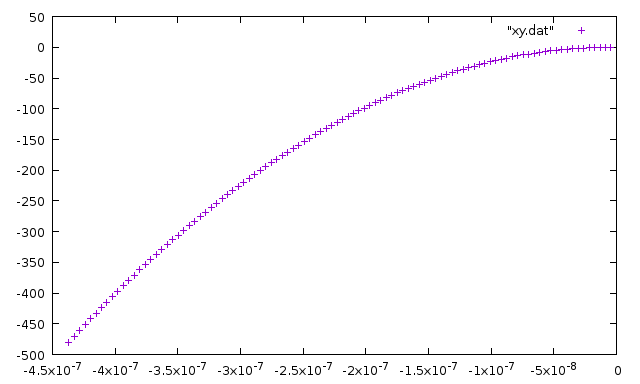
\includegraphics[width=\linewidth]{xy.png}
  \caption{xy.}
  \label{fig:xy}
\end{figure}




\pagebreak
Al adquirir estos conocimientos procedimos a realizar un código más complicado en el cual se nos pedía calcular dichos tiros parabólicos pero con una velocidad inicial (Vo) dada y también realizar los cálculos con los ángulos en aumento progresivo de 15 grados comenzando con 15 grados hasta llegar a 90 grados. De igual forma debíamos expulsar datos a una archivo de texto y posteriormente graficarlos en Gnuplot.

El código quedó de la siguiente manera:
\begin{verbatim}
!desplazamiento en X & Y

 implicit none
 !Declaramos Constantes
 Real,Parameter:: Pi=3.1415927
 Real,parameter:: g=10
 Real, parameter:: delt=0.1
 Real,parameter::Vo=10
 Integer::k
 Integer::l
 !declaramos Variables
 Real::t,U
 real::x,y
 

print*, "calcularemos las cordenas del tiro parabólico"
open(1, file='final.dat',status='unknown')
do l=15,90,15
   U=float(l)*pi/180.0
   write(1,*) ''

Do k=1,100
    t=float(k)*delt
    x =Vo*(cos(u))*t
    y= Vo*sin(u)*t-(0.5)*(g)*(t*t)
    
    if (y<0.0)  exit
    
     write(1,*) x,y
  end do
  end do
  close(1)
\end{verbatim}
Los gráfica de los datos obtenidos se muestran en la Figura2 (Figure2:final)
\begin{figure}[h!]
  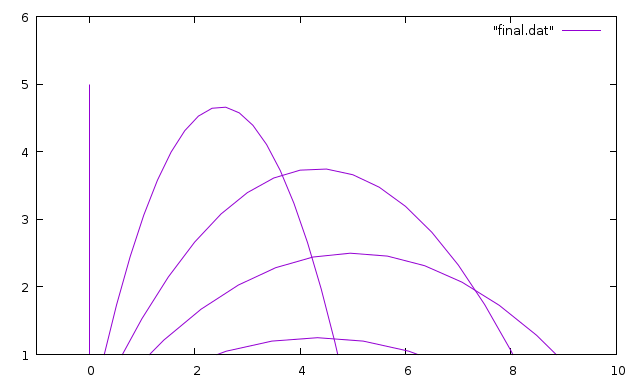
\includegraphics[width=\linewidth]{final.png}
  \caption{final}
  \label{fig:boat1}
\end{figure}

\section{conclusión}
Gracias a esta práctica se logró obtener el conocimiento y práctica de los comandos Do,IF,Open (en caso de querer escribir los datos en un block de notas, así como funcionamiento del graficador Gnuplot.

\section{Bibliografia}
\begin{verbatim}
http://computo.fismat.umich.mx/mn1/tutor_fort/loops.html
http://computo.fismat.umich.mx/mn1/tutor_fort/if.html
https://www.latex-tutorial.com/tutorials/beginners/latex-figures/
http://ocw.um.es/gat/contenidos/ldaniel/ipu_docs/latex/tema6.html
http://gnuplot.info/
\end{verbatim}


\end{document}
